\chapter{Introduction}\label{ch.intro}
\section{first section}\label{sec.intro1}

This template was written in \parencite{lamport1994latex}. 
This is \autoref{sec.intro1} of \autoref{ch.intro}. Dipoles are so good. Look at  the dipole in \autoref{fig.intro1}. This stuff is really important in . In fact, dipoles explain  signal generation.

\begin{figure}[H]
    \centering
    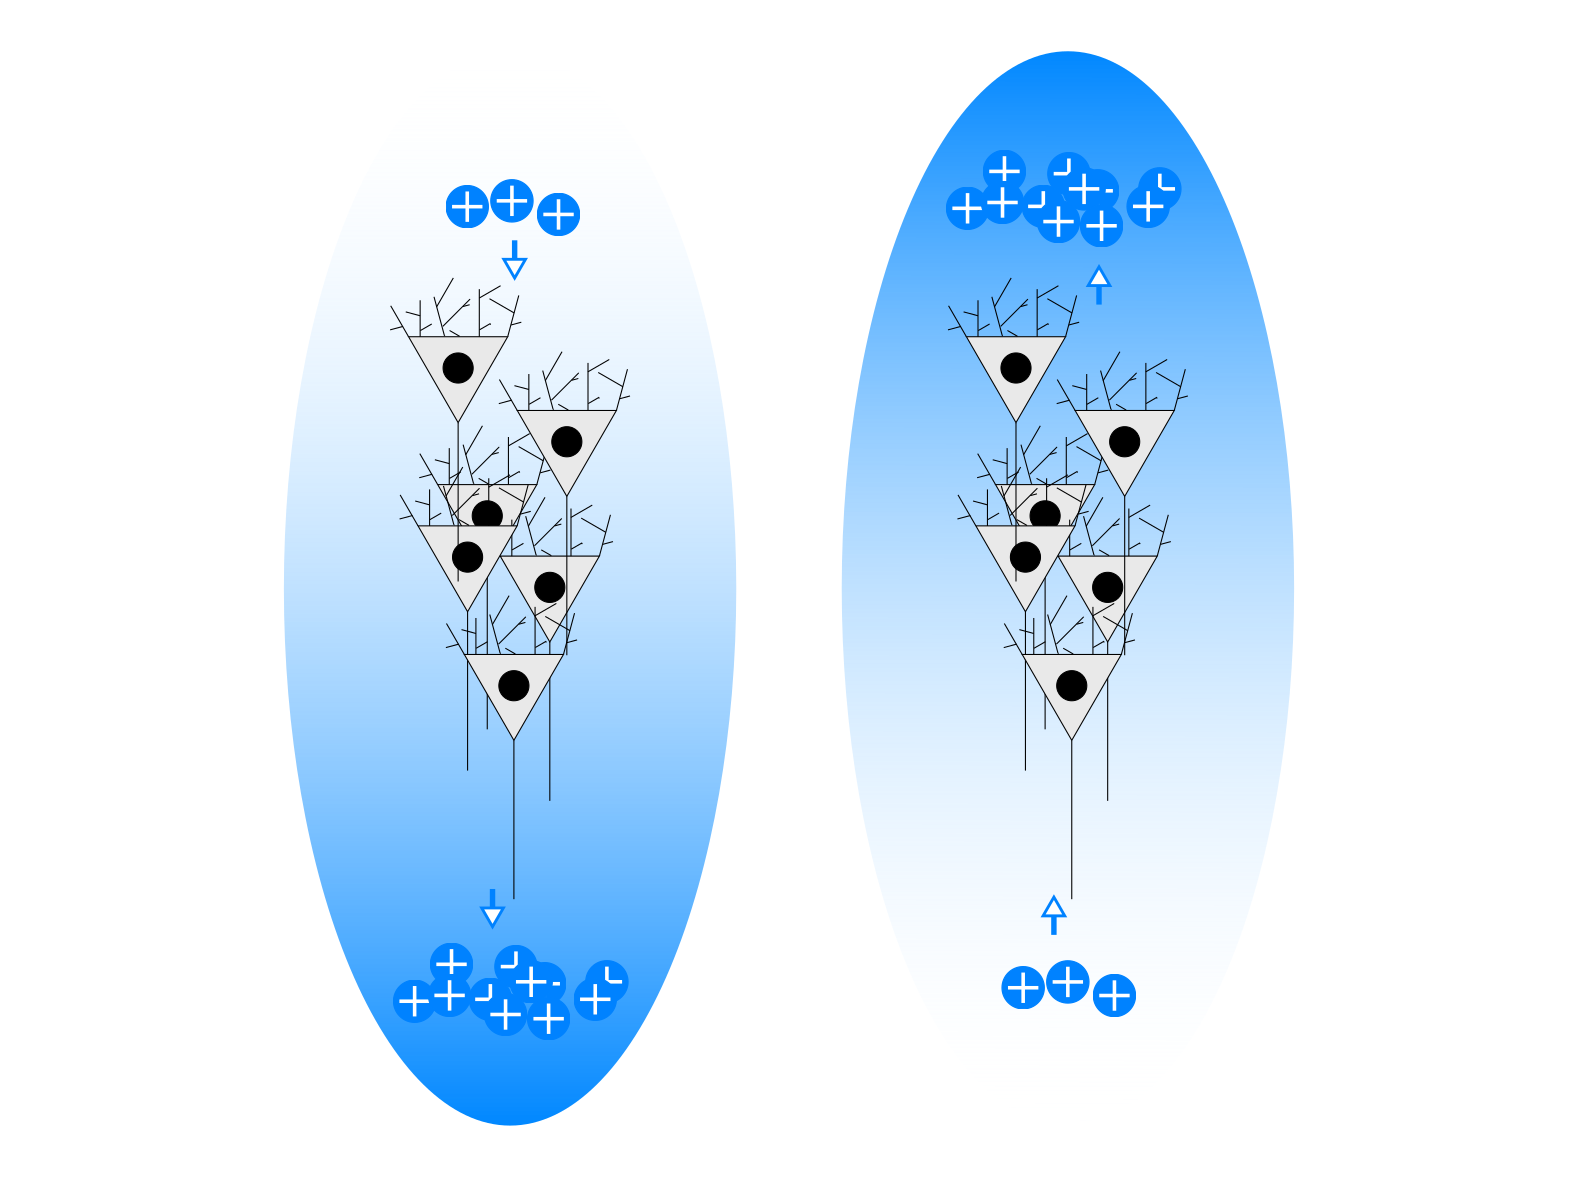
\includegraphics[width=0.9\linewidth,frame]{Thesis/Manuscript/Images/BodyMatter/Introduction/dipole.png}
    \caption[figure title]{figure title}
    \label{fig.intro1}
\end{figure}




\section{Hypothesis}
\begin{itemize}
    \item[\textbullet] 
\end{itemize}


\section{Objectives}

\subsection{General objective}
\begin{itemize}
    \item[\textbullet] 
\end{itemize}


\subsection{Specific objectives}
\begin{itemize}
    \item[\textbullet] 
    
    \item[\textbullet] 
    \item[\textbullet] 
\end{itemize}




